\documentclass[notheorems,serif,table,compress]{beamer}  %dvipdfm选项是关键,否则编译统统通不过
%%------------------------常用宏包------------------------
%%注意, beamer 会默认使用下列宏包: amsthm, graphicx, hyperref, color, xcolor, 等等
\usepackage{fontspec,xunicode,xltxtra}  % for XeTeX
\usepackage{verbatim}
\usepackage{mathabx}
\usepackage{latexsym}
\usepackage{amsfonts,amssymb}
\usepackage{styles/iplouclistings}
\usepackage{fancybox}
\usepackage{colortbl}
\usepackage{tcolorbox}
%\usepackage[T1]{fontenc}
%\usepackage{bookman}
\usepackage{subfigure}
\usepackage{hyperref}
\usepackage{listings}
\usepackage{animate}
\usepackage[absolute,overlay]{textpos}
\usepackage{graphicx}
\usepackage{tikz}
\usepackage[americaninductors,europeanresistors]{circuitikz}
\usepackage{tikz}
\usepackage{fancybox}     %% 定义zhushadow时用到
\usepackage{pifont} %ding用到
\newsavebox{\mysaveboxOne}  %%为了在only中使用lstlisting
\newsavebox{\mysaveboxTwo}
\newsavebox{\mysaveboxThree}
\newsavebox{\mysaveboxFour}
\newsavebox{\mysaveboxFive}
\newsavebox{\mysaveboxSix}
\newsavebox{\mysaveboxSeven}
\newcommand\zhushadow[2][purple]{\hskip5pt\shadowbox{\color{#1}\small\kai #2\vspace{3mm}}}

%%------------------------ThemeColorFont------------------------
%% Presentation Themes
% \usetheme[<options>]{<name list>}
%\usetheme{Madrid}
\usetheme{Berkeley}
%% Inner Themes双精度计算
% \useinnertheme[<options>]{<name>}
%% Outer Themes
% \useoutertheme[<options>]{<name>}
%\useoutertheme{miniframes} 
%% Color Themes 
%\usecolortheme[<options>]{<name list>}
%% Font Themes
\usefonttheme{serif}
\setbeamertemplate{background canvas}[vertical shading][bottom=white,top=structure.fg!7] %%背景色, 上25%的蓝, 过渡到下白.
\setbeamertemplate{theorems}[numbered]
\setbeamertemplate{navigation symbols}{}   %% 去掉页面下方默认的导航条.
\usepackage{styles/zhfontcfg}
%\setsansfont[Mapping=tex-text]{文泉驿正黑}  %% 需要fontspec宏包
     %如果装了Adobe Acrobat,可在font.conf中配置Adobe字体的路径以使用其中文字体
     %也可直接使用系统中的中文字体如SimSun,SimHei,微软雅黑 等
     %原来beamer用的字体是sans family;注意Mapping的大小写,不能写错
     %设置字体时也可以直接用字体名,以下三种方式等同:
     %\setromanfont[BoldFont={黑体}]{宋体}
     %\setromanfont[BoldFont={SimHei}]{SimSun}
     %\setromanfont[BoldFont={"[simhei.ttf]"}]{"[simsun.ttc]"}
%%------------------------MISC------------------------
\graphicspath{{figures/}}         %% 图片路径. 本文的图片都放在这个文件夹里了.
%%------------------------listing------------------------
%\lstset{language=[LaTeX]TeX,Python}
%%------------------------正文------------------------
\begin{document}
\XeTeXlinebreaklocale "zh"         % 表示用中文的断行
\XeTeXlinebreakskip = 0pt plus 1pt % 多一点调整的空间
%%----------------------------------------------------------
%% This is only inserted into the PDF information catalog. Can be left
%% out.
%%%
%% Delete this, if you do not want the table of contents to pop up at
%% the beginning of each subsection:
%\AtBeginSection[]{                              % 在每个Section前都会加入的Frame
%  \frame<handout:0>{
%    \frametitle{Contents}\small
%    \tableofcontents[current,currentsubsection]
%  }
%}
%
%\AtBeginSubsection[]                            % 在每个子段落之前
%{
%  \frame<handout:0>                             % handout:0 表示只在手稿中出现
%  {
%    \frametitle{Contents}\small
%    \tableofcontents[current,currentsubsection] % 显示在目录中加亮的当前章节
%  }
%}

\setbeamertemplate{caption}{\raggedright\insertcaption\par}

%%----------------------------------------------------------
\logo{
\includegraphics[scale=0.13]{ouclogo.png}}
\title{数字图像处理学习}
%\subtitle{Bottom-Up Saliency Detection Model Based on Human Visual Sensitivity and Amplitude Spectrum}
\subtitle{第三章}
\author[]{\textcolor{olive}{常琳}}
\institute[CVBIOUC]
{
\small\textcolor{violet}{CVBIOUC\\
%Ocean University of China\\
\url{http://vision.ouc.edu.cn/~zhenghaiyong}}
}
%\date[]{}
%\titlegraphic{
%\includegraphics[height=1.0cm]{ouc-logo.jpg}}
\frame{ \titlepage }
%%----------------------------------------------------------
%\section*{Contents}
\frame{\frametitle{Contents}\tableofcontents}
%%----------------------------------------------------------
\def\hilite<#1>{\temporal<#1>{\color{blue!15}}{\color{black}}{\color{black}}}
\newcommand{\shadow}[2][purple]{\hskip5pt\shadowbox{\color{#1}\small \kai #2\vspace{3mm}}}
\newcommand{\colorrbox}[2][purple]{\doublebox{\color{#1}\small \kai#2}}

%============================================================================

\section{灰度变换}

%==========================================================================


\begin{frame}[fragile]
\frametitle{灰度变换}
灰度变换在图像的单个像素上操作,主要以对比度和阈值处理为目的。空间性能涉及改
善性能的操作。

空间域处理由下式表示:
\begin{equation} \label{3.1}  %这里应该如何写label里面的标号?
g(x,y)=T[f(x,y)]
\end{equation}
最小领域的大小为$1*1$时,变换函数可以写为:
\begin{equation} \label{3.2}  
 s=T(r) 
\end{equation}
\end{frame}


\subsection{灰度变换函数}

\begin{frame}
\frametitle{灰度变换函数}
 图像增强常用三种基本函数:线性函数、对数函数、幂律函数
 \begin{description}
 \item [线性函数 imadjust]
 \end{description}
 \begin{figure}[!ht]
  \begin{minipage}[t]{0.4\textwidth}	
  \centering
  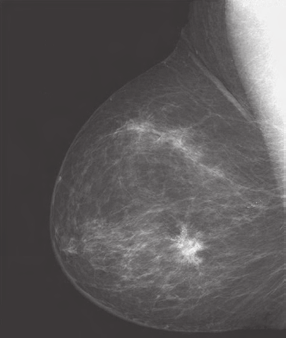
\includegraphics[width=1.5in]{imadjust_a.png}
  \caption{图1(a)}
  \end{minipage}
  \begin{minipage}[t]{0.4\textwidth}
  \centering
  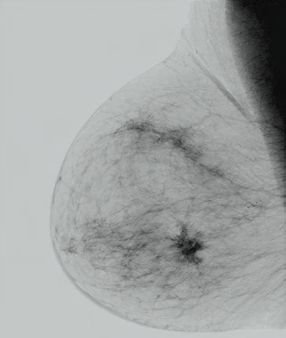
\includegraphics[width=1.5in]{imadjust_b.png}
  \caption{图1(b)}
  \end{minipage}
  \end{figure} 
使用该函数可由图1(a)得到明暗反转的图像,如图1(b)。
\end{frame}
 

\begin{frame}
\frametitle{灰度变换函数}
    
\begin{description}
 \item [对数变换函数im2uint8]
 \end{description}
    \begin{figure}
        \begin{minipage}[t]{0.4\linewidth}
        \centering
        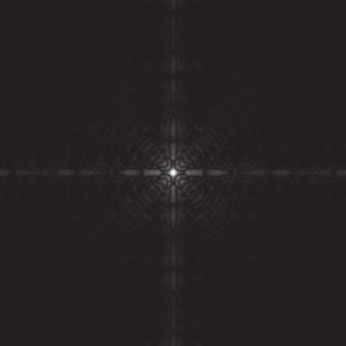
\includegraphics[width=1\linewidth]{ma2_a.png} 
        \caption{图2(a)}
        \end{minipage}
        \begin{minipage}[t]{0.4\linewidth}
        \centering
        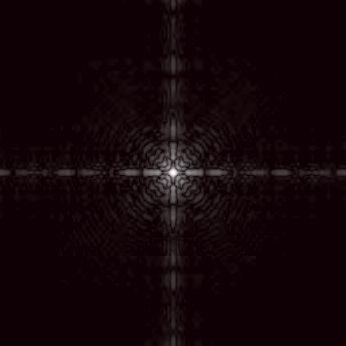
\includegraphics[width=1\linewidth]{ma2_b.png} 
          \caption{图2(b)}
        \end{minipage}
    \end{figure}
对数变换函数压缩值的范围,改进细节的丰富程度,原图图2(a),改进后如图2(b)。
\end{frame}

\subsection{直方图处理}
 \begin{frame}
\frametitle{直方图处理}
    \begin{itemize}
        \item 与$r_{k}$相对的$p_{r}(r_{k})$图形通常称为直方图。
        \item 直方图操作可用于图像增强。
     \end{itemize}
     直方图均衡和直方图匹配
    
 \end{frame}

\begin{frame}
\frametitle{直方图均衡}
   作用:使图像的灰度级跨越更宽的灰度范围,增强对比度。
   灰度级范围为 [0,L-1] 的数字图像的直方图是离散函数 $h(r_{k})=n_{k}$ 。
   离散函数主要通过以下两个公式实现直方图均衡:
   \begin{equation}    \label{3.8} %????
    p_{r}(r_{k})= \frac{n_{k}}{MN},k=0,1,2\ldots,L-1
   \end{equation}

   \begin{equation} \label {3.9}
     s_{k}=T(r_{k})=(L-1)\sum_{j=0}^{k}p_{r}(r_{j})=\frac{(L-1)}{MN} \sum_    {j=0}^{k}{n_{j}},k=0,1-2\ldots,L-1
   \end{equation}
 \end{frame}
 直方图均衡化实现函数:histeq
 图3(a)为花粉图像原图,图3(b)为使用histeq函数后的结果。
 \begin{figure}
        \begin{minipage}[t]{0.4\linewidth}
        \centering
        
\includegraphics[width=1\linewidth]{huafen_a.png} 
        \caption{图3(a)}
        \end{minipage}
        \begin{minipage}[t]{0.4\linewidth}
        \centering
        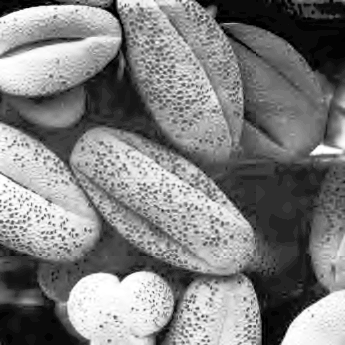
\includegraphics[width=1\linewidth]{huafen_c.png} 
          \caption{图3(b)}
        \end{minipage}
    \end{figure}
从图3(b)可以看出,直方图均衡化后,平均亮度以及对比度都有所增强。

 \begin{frame}
\frametitle{直方图匹配(规定化)}
    
\begin{description}
 \item [性质]能自动地确定变换函数,该函数寻求产生有均匀直方图的输出图像。
 \item [用途]当需要自动增强时。
 \item [优点]结果可预知,实现简。
 \end{description}

主要公式:
 \begin{equation} \label {3.13}
s_{k}=T(r_{k})=(L-1)\sum_{j=0}^{k}p_{r}(r_{j})=\frac{(L-1)}{MN}\sum_{j=0}^{k}{n_{j}},k=0,1,2\ldots,L-1
\end{equation}
 
  \begin{equation} \label {3.14}
G(z_{q})=(L-1)\sum_{i=0}^{q}p_{z}(z_{i})
\end{equation}
(任何$p_{z}(z_{i})$都不能为0)
\end{frame}
\begin{frame}
\frametitle{直方图匹配(规定化)}
\begin{equation} \label {3.15}
G(z_{q})=s_{k}
\end{equation}
$p_z(z_{i})$是规定的直方图的第i个值
\begin{equation} \label {3.16}
z_{q}=G^{-1}(s_{k})
\end{equation}
\end{frame}

\begin{frame}
\frametitle{直方图匹配(规定化)}
  直方图匹配的主要步骤:
  \begin{enumerate}
  \item 计算$p_{r}(r)$,计算$s_{k}$并四舍五入为$[0,L-1]$内的整数。
  \item 用$p_{z}(z_{i})$计算变换函数$G$的所有值,把$G$四舍五入为$[0,L-1]$内的整数。
  \item 对每一个$s_{k},k=0,1,2\ldots,L-1$,使用$G$值寻找相应的$z_{q}$值,使$G(z_{q})$最接近$s_{k}$,当满足给定$s_{k}$的$z_{q}$值多余一个时,选最小的$z_{q}$
  \item 把该图像中的每个均衡后的像素值$s_{k}$映射为直方图规定化后的图像中的相应$z_{q}$值,形成直方图规定化后的图像。
   \end{enumerate} 

 \end{frame}
%=======================================================================
\begin{frame}
\frametitle{在图像增强中使用直方图统计}
 
 求均值和方差
 \begin{description}
 \item [均值]是平均灰度的度量,也是划分某一区域灰度强弱的标准。
 \item [方差]是图像对比度的度量,也是划分某一区域对比度强弱的标准。
 \item [局部增强]中,局部均值和方差是根据图像中每一像素的邻域内的图像特征进行改变的基础。
 \end{description}
 
 \end{frame}
%========================================================================
\section{空间滤波}
\subsection{空间滤波基础}
\begin{frame}
\frametitle{空间滤波基础}
 
 \begin{description}
 \item [空间滤波器]由(1)一个邻域,(2)对该邻域包围的图像像素执行的预定义操作组成)。
 \end{description}
 使用大小为$m*n$的滤波器对大小为$M*N$的图像进行线性空间滤波,可由下式表示:
\begin{equation} \label {3.13}
g(x,y)=\sum_{s=-a}^{a}\sum_{t=-b}^{b}w(s,t)f(x+s,y+t)
\end{equation}
 \end{frame}

\begin{frame}
\frametitle{空间滤波基础}
 相关与卷积的概念
 \begin{description}
 \item [相关]滤波器模板移过图像并计算每个位置乘积之和。
 \item [卷积]滤波器先旋转$180^{o}$
 \end{description}
 
 \end{frame}

\begin{frame}
\frametitle{空间滤波器模板的产生}
 生成大小为$m*n$的线性空间滤波器,要求根据该滤波器支持什么样的操作指定模板系数。
线性滤波能进行的操作:乘积求和 
 
 \end{frame}

\subsection{平滑空间滤波器}

\begin{frame}
\frametitle{平滑线性滤波器}
 \begin{description}
 \item [平滑线性滤波器]平滑线性滤波器使用滤波器模板确定的邻域内像素的平均值代替图像中每个像素的值,降低了图像灰度的“尖锐”变化,也叫均值滤波器。
 \end{description}

主要应用:去除某些与模板器尺寸相比较小的像素区域。

 均值与加权平均(一些像素的重要性比另一些像素的重要性要大)
 \end{frame}

\begin{frame}
\frametitle{统计排序(非线性)滤波器}
 使用统计排序结果决定的值代替中心像素的值。
 其中中指滤波器可以很好的处理脉冲噪声。(medfilt2函数)
 \end{frame}

\subsection{锐化空间滤波器}
\begin{frame}
\frametitle{锐化空间滤波器}
 \begin{description}
 \item [锐化处理]的主要目的是突出灰度的过度部分。
 \item [实现方法]微分。
 \end{description}
 
 \end{frame}

\begin{frame}
\frametitle{锐化空间滤波器}
 一维函数一阶微分
\begin{equation}
 \frac{\partial f}{\partial x}=f(x+1)-f(x)
\end{equation}
 一维函数二阶微分
\begin{equation}
 \frac{\partial^{2}f}{\partial x^{2}}=f(x+1)+f(x-1)-2f(x)
\end{equation}
 二阶微分在增强细节方面比一阶微分好。
 \end{frame}

\begin{frame}
\frametitle{使用二阶微分进行图像锐化——拉普拉斯算子}
 二维图像函数$f(x,y)$拉普拉斯算子为:
\begin{equation}
\bigtriangledown^{2}f= \frac{\partial^{2}f}{\partial x^{2}}+\frac{\partial^{2}f}{\partial y^{2}}
\end{equation}
实现拉普拉斯算子可用滤波模板。

微分算子强调图像中灰度的突变而不是缓慢变化。
 \end{frame}

\begin{frame}
\frametitle{使用二阶微分进行图像锐化——拉普拉斯算子}
 用拉普拉斯算子对图像增强的方法是将原图像和拉普拉斯图像叠加,公式如下:
\begin{equation}
g(x,y)=f(x,y)+c[\bigtriangledown^{2}f(x,y)]
\end{equation}
 \end{frame}




%===============================================================================


\end{document}
